%%%%%%%%%%%%%%%%%%%%%%%%%%%%%%%%%%%%%%%%%%%%%%%%%%%%%%%%%%
% intro.tex
%%%%%%%%%%%%%%%%%%%%%%%%%%%%%%%%%%%%%%%%%%%%%%%%%%%%%%%%%%


\begin{figure}
\begin{center}
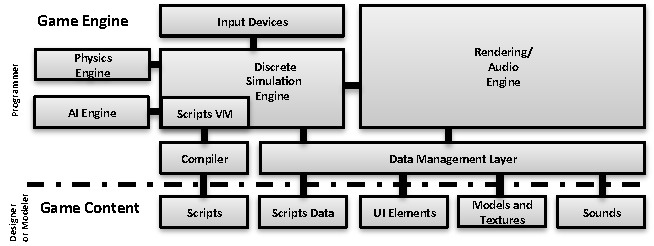
\includegraphics[scale=0.8]{engine_architecture.pdf}
\end{center}
\label{fig:data_driven_games}
\caption{Data-driven engine architecture, from \cite{SGL}}
\end{figure}

Virtual reality browsers face big challenges centered on performance and complexity. Performance is needed because the framerate at which the virtual world is rendered and animated must be high enough to give the user a feeling of smoothness. The scene must be rendered at least at 30 frames per seconds, but higher framerates (e.g. 60 frames per second) are perceived by the user as more pleasant.

Both the visual and logical complexities of a virtual world are very important. Visual richness gives the user the impression of a more realistic and detailed world, with many beautifully rendered objects, while logical complexity permits articulated responses that give the user the feeling of being part of a realistic world with its own set of rules and internal laws.

One of the most important tasks for developers of interactive worlds is to find the right trade-off between these sometimes conflicting requirements. Increasing performance requires a mixture of compromise (reducing the size of the world or ``dumbing down'' its responses) and time-consuming low-level optimization. We believe that automated optimization of interactive applications is a fundamental frontier if we wish to enable developers to build richer worlds without exponentially increasing costs.

Modern 3D browsers and engines are based on a data-driven architecture as shown in Figure \ref{fig:data_driven_games}, taken from \cite{SGL}.

In a data-driven engine the engine contains only general knowledge about virtual worlds, but nothing specific about the peculiar features of a specific virtual world. The specific virtual world will be loaded from the game content in the form of configuration files and scripts. A data-driven engine loads from files two main datasets:

\begin{itemize}
\addtolength{\itemsep}{-0.5\baselineskip}
\item a \textbf{scene}, the set of entities that populate the virtual world
\item \textbf{scripts}, the set of (possibly complex) behaviors that animate the scene entities
\end{itemize}

The scene is composed by a heterogeneous set of entities, each of a different kind. Entities may be virtual characters, trees, 2d or 3d models; entities may also be purely logical and invisible entities such as timers, triggers and proximity sensors.

Scripts give depth to a scene by implementing complex interrelationships between entities. Scripting can be done at three different levels of increasing complexity and expressive power:

\begin{itemize}
\addtolength{\itemsep}{-0.5\baselineskip}
\item \textit{routing} is a simple transmission of values from one entity to another
\item more complex scripts can perform data conversions when moving information between entities
\item even more advanced scripts can create, remove or modify entities of a scene
\end{itemize}

The usual implementation of an engine (see \cite{GAME_OO_HIERARCHY}) features an object-oriented architecture of classes. At the root of this architecture is a class that represents the most generic entity, and from which all other entities are derived. The engine maintains a list of these generic entities, which are all updated and handled through a set of virtual functions. This architecture is a source of often underestimated overhead. Dynamic dispatching is not too costly for a few calls, but when we have many entities, the cost of invoking various virtual functions many times for each frame can become very high. Sometimes the cost of the dynamic dispatching architecture may become higher than the cost of the actual operations being dispatched.

Scripts usually access the scene dynamically. This means that a script must look for the right entities with a mixture of lookups by name and unsafe casts. For example, consider how a Java script may access the \texttt{time} field of a \texttt{myClock} node of type \texttt{timer}:

\begin{lstlisting}
\addtolength{\itemsep}{-0.5\baselineskip}
X3DNode myClock = 
 mainScene.getNamedNode("myClock");
SFTime time = 
  (SFTime) myClock.getField("time");
\end{lstlisting}

This style is unsafe, since \texttt{myClock} may not exist or it may have the wrong type, and it also incurs in significant overhead.

In this paper we will focus exclusively on the X3D language, since it is a recognized standard and it offers a good benchmark to test virtual worlds where we can specify our scene and its various scripts. In the paper we show how we have tackled the problem of increasing performance in X3D browsers while also making scripts safe. We have used a simple compilation technique that removes many unnecessary dynamically dispatched invocations; this technique also allows us to introduce safety for scripts that access the state, so that they do not need to perform unsafe dynamic lookups when searching for specific nodes. To the best of our knowledge, this is the first approach that experiments with compiling X3D scripts and scenes in order to achieve greater performance and safe scripts. None of the previous approaches we are aware of focuses on compilation of X3D as a means to achieve both higher performance (by reducing overhead) and safety (by introducing compile-time checks). Higher performance through compilation includes a long list of research work such as \cite{OPT1,OPT2,OPT3} which has shown that compilation can yield better runtime performance by reducing dynamic overhead and improving other properties of the generated code. Similarly, introducing safety in dynamic languages such as scripting systems has been studied in general in the context of generating typed programs from untyped scripts in \cite{SAFESCRIPTS1}, and the problem of statically typing information which is generally untyped has also been explored in the Haskell community in \cite{SAFESCRIPTS2} among many others.

In Section \ref{sec:solution_workflow} we discuss the general architecture of our system. In Section \ref{sec:compiling_scene} we show how our technique generates the code and the type definitions that represent a scene. In Section \ref{sec:case_study} we show an example of a compiled scene and its routes. In Section \ref{sec:benchmarks} we report some benchmarks that show speed increasing when rendering a sample scene with just nodes and routes by applying our technique. Finally, in Section \ref{sec:compiling_scripts} we discuss how we represent scripts that externally access the scene.

